\documentclass[12pt]{article}

\usepackage{classDM}
\usepackage{hyperref}
\usepackage[normalem]{ulem}
\usepackage{float}
\usepackage{tabu}

\title{Gender Roles in English Movies}
\author{Rebeka Mukherjee, Archit Rathore, Yash Gangrade}
\date{April 15, 2019}

\begin{document}
\maketitle

\section{Introduction}
Gender refers to the socially constructed characteristics of women and men such as norms, roles and interpersonal relationships \cite{gender_definition}. The United Nations recognizes gender equality not only as a fundamental human right, but also a necessary foundation for a `peaceful, prosperous and sustainable world' \cite{gender_equality}. Achieving gender equality is one of UN's goals towards sustainable development. \\

Media plays an important role in our lives. Though not an accurate representation, but media largely reflects the social constructs of the world we live in. At the same time, media largely influences our daily decisions and way of living. One of the most influential forms of media in the modern world is movies. We speculate that the representation of the genders on screen largely reflects our perceptions of the genders in real life. \\

In this study we explored and analyzed the role of gender in movies. Our main objective was to compare our findings with the current situation of gender equality in the real world. This comparison would allow us to answer questions like: how can media be used efficiently to achieve equality among the genders? \\

The following sections describe our project in detail. Section 2 provides information about the data that we used for the project, how we processed it for the study, and the preliminary exploration done on it. Section 3 focuses on the approaches taken by us to meet the project objective. The findings of the approaches are reported in section 4. Section 5 documents the evaluations of these findings. Section 6 and 7 touch up on the future directions of this project and the conclusions we drew from this project, respectively.

\section{Data}
The complete data is fetched from this Kaggle dataset: \url{https://www.kaggle.com/rounakbanik/the-movies-dataset/}. The dataset is downloadable after creating a Kaggle account and comes with a public domain creative commons license. \\

The dataset contains metadata for 45,000 movies. Data points include cast, crew, plot keywords, budget, revenue, posters, release dates, languages, production companies, countries, TMDB vote counts and vote averages. The compressed dataset is roughly 230 MBs. \\

We also developed a web scraper to extract the script of these movies from the Internet Movie Script Database (IMSDB) website: \url{https://www.imsdb.com/}.

\subsection{Data Processing}
Though the downloaded data was in CSV format, there were some issues with the structure such as... We created objects for each movie by using information from the files `movies\_metadata.csv' and `credits.csv'. Figure \ref{movie} shows all the member variables and methods associated with each object. We used these collection of objects for all preliminary data exploration. \\

\begin{figure}[H]
\begin{center}
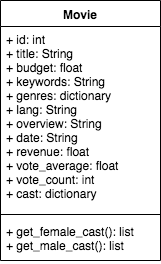
\includegraphics[width=2in]{movie_class_diagram.png}
\end{center}
\caption{Class diagram for the Movies class}
\label{movie}
\end{figure}

We also wanted to convert the data into a graph that could be further used to perform spectra based analysis methods. For this purpose, we randomly selected 300 English movies whose script was available in the IMSDB website. The reason we selected only English movies is because we speculate that it is the language in which most number of movies are viewed in the United States. English movie scripts were also easily available from the IMSDB website, and easy for us to process and analyze.\\

We came up with a list of gender words (Table \ref{gender_words}) and created a bag of words vector for each of these movies based on how many times these words appeared in the script for that movie. Table \ref{bow_vectors} shows the corresponding vectors for a subset of 3 movies. \\

\begin{table}
\begin{center}
\begin{tabu} to 0.6\textwidth { | X[c] | X[c] | }
\hline
\textbf{Male Words} & \textbf{Female Words} \\ \hline
he & she \\
him & her \\
his & hers \\
himself & herself \\
man & woman \\
boy & girl \\
lord & lady \\
sir & madam \\
father & mother \\
grandfather & grandmother \\
son & daughter \\
grandson & granddaughter \\
brother & sister \\
husband & wife \\
boyfriend & girlfriend \\
uncle & aunt \\
nephew & niece \\ \hline
\end{tabu}
\end{center}
\caption{Gender words used to generate bag of words vectors}
\label{gender_words}
\end{table}

\begin{table}
\begin{center}
\begin{tabu} to \textwidth { | X[c] | X[c] | }
\hline
\textbf{Movie Name} & \textbf{BOW Vector} \\ \hline
Toy Story & [158, 86, 220, 27, 14, 13, 0, 4, 0, 0, 1, 0, 0, 0, 0, 0, 0, 11, 25, 0, 0, 0, 0, 1, 0, 6, 0, 0, 0, 3, 1, 0, 0, 0] \\ \hline
Braveheart & [411, 184, 494, 17, 45, 15, 41, 13, 60, 0, 32, 0, 17, 16, 0, 12, 7, 145, 187, 1, 6, 10, 12, 4, 1, 9, 0, 7, 0, 0, 9, 0, 0, 0] \\ \hline
Notting Hill & [181, 50, 68, 5, 31, 3, 1, 10, 0, 0, 1, 0, 2, 0, 6, 0, 0, 152, 104, 1, 2, 8, 22, 1, 1, 3, 2, 0, 0, 2, 2, 1, 0, 0] \\ \hline
\end{tabu}
\end{center}
\caption{Bag of words vector generated for 3 movies.}
\label{bow_vectors}
\end{table}

We found the pairwise similarities between two movies by taking the cosine similarity (1 - cosine distance) between the bag of word vectors for the corresponding movies. Then we represented all the movies as an undirected graph by constructing an adjacency matrix where each movie was a vertex, and the weight of the edges between them was their pairwise similarity. We had to additionally adjust the adjacency matrix by setting the diagonal elements to 0. Table \ref{adjacency_matrix} shows the adjacency matrix created from the movies mentioned in Table \ref{bow_vectors}.

\begin{table}
\begin{center}
\begin{tabu} to \textwidth { | X[c] | X[c] | X[c] | X[c] | }
\hline
 & \textbf{ToyStory} & \textbf{Braveheart} & \textbf{Notting Hill} \\ \hline
\textbf{ToyStory} & 0 & 0.975 & 0.668 \\ \hline
\textbf{Braveheart} & 0.975 & 0 & 0.817 \\ \hline
\textbf{Notting Hill} & 0.668 & 0.817 & 0 \\ \hline
\end{tabu}
\end{center}
\caption{Adjacency matrix generated for the above 3 movies.}
\label{adjacency_matrix}
\end{table}

\subsection{Data Exploration}
We found out that out of 32937 English movies, only 4457 \textbf{(13.53\%)} movies had a cast where the number of female cast members were more than the number of male cast members. \\

Next, wanted to find out the female-to-male ratio for each genre of movie. To do this we simply extracted all the genres of English movies and for each genre, we found the ratio of the number of female cast members to the number of male cast members for every movie in that genre. Then we took the mean of the ratios for every movie in a particular genre. Table \ref{genre_female_male_ratio} shows the results that we found from this step.

\begin{table}[H]
\begin{center}
\begin{tabu} to 0.6\textwidth { | X[c] | X[c] | }
\hline
\textbf{Genre} & \textbf{Female-to-male Ratio} \\ \hline
Action &  0.395 \\
Adventure & 0.425 \\
Animation & 0.457 \\
Comedy & 0.675 \\
Crime & 0.479 \\
Documentary & 0.155 \\
Drama & 0.678 \\
Family & 0.689 \\
Fantasy & 0.607 \\
Foreign & 0.521 \\
History & 0.324 \\
Horror & 0.678 \\
Music & 0.6 \\
Mystery & 0.652 \\
Romance & 0.814 \\
Science Fiction & 0.494 \\
TV Movie & 0.877 \\
Thriller & 0.595 \\
War & 0.295 \\
Western & 0.319 \\ \hline
\end{tabu}
\end{center}
\caption{Female-to-male cast ratios for each genre of English movies.}
\label{genre_female_male_ratio}
\end{table}

It is very surprising to see that `Documentary' movies have the least female-to-male ratio, followed closely by `War' and `Western' movies, which is not so surprising. On the other hand, `TV Movies' have the largest female-to-male ratio, followed by `Romance' and `Family'. \\

We also wanted to find out the female-to-male ratio according to language of the movie. To do this we extracted the languages of all movies and for each language, we found the ratio of the number of female cast members to the number of male cast members for every movie in that language. Then we took the mean of the ratios for every movie in a particular language. While doing this we ignored any language that had less than 5 movies in the dataset. Table \ref{genre_female_male_ratio} shows the results for the top 20 movies with the highest female-to-male ratios. \\

Vietnamese movies apparently have the largest female-to-male cast ratio which is quite close to gender equality, followed by Tagalog and Korean movies. Surprisingly, all the three languages are from East Asian countries. 

\begin{table}[H]
\begin{center}
\begin{tabu} to 0.6\textwidth { | X[c] | X[c] | }
\hline
\textbf{Language} & \textbf{Female-to-male Ratio} \\ \hline
Vietnamese (vi) & 0.994 \\
Tagalog (tl) & 0.787 \\
Korean (ko) & 0.72 \\
French (fr) & 0.682 \\
Latin (la) & 0.667 \\
Esperanto (eo) & 0.667 \\
Kurdish (ku) & 0.667 \\
Spanish (es) & 0.653 \\
Abkhazian (ab) & 0.648 \\
Japanese (ja) & 0.639 \\
Italian (it) & 0.623 \\
Hindi (hi) & 0.606 \\
Swedish (sv) & 0.596 \\
German (de) & 0.594 \\
English (en) & 0.566 \\
Catalan (ca) & 0.546 \\
Portuguese (pt) & 0.546 \\
Chinese (zh) & 0.54 \\ \hline
\end{tabu}
\end{center}
\caption{Top 20 languages with the highest female-to-male cast ratios.}
\label{lang_female_male_ratio}
\end{table}

\section{Methods}

What is the key idea your project is built upon? If there is no interesting ideas, I will be a little disappointed. This should describe the rational behind and what you were hoping to discover about the different approaches you are comparing, or what extension you are proposing to a existing technique, or how you are applying a technique to a dataset where it has not been explored before. State this clearly in the beginning; try to make me excited to read the remainder of your report to find out how your idea played out!

Explain what you did. Did you prove something? Did you implement something? Did you compare several things? Did you extend something? \\

We tried 3 different methods to prove our objective.

\subsection{Approach 1: Regression}
Our first approach was to see if we could fit a least squares linear regression model to our data. We wanted to predict the female-to-male cast ratio of English movies, given the year the movie was released. To do this we found the female-to-male cast ratio for each movie released in a particular year. Then, for each year we found the mean of these ratios. We used the method \textbf{LinearRegression()} from the Python package \textbf{sklearn} to fit our data.

\subsection{Approach 2: }

\subsection{Approach 3: Spectral Clustering}


\section{Results}

Explain what you learned. This is often greatly aided through charts of experiments. But you should also include what lessons you came away with in words; just charts or mathematics is insufficient.

\subsection{Approach 1: Regression}

Figure \ref{regression} shows a plot of the female-to-male cast ratio against the corresponding year using blue points. It also shows the linear regression model that was fit on the data points using a red line. We can see that the ratio increases steadily with each year.

\begin{figure}[H]
\begin{center}
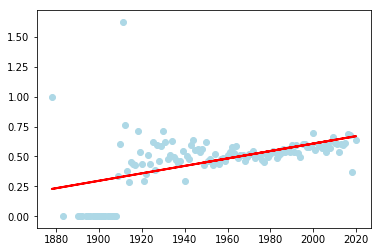
\includegraphics[width=4in]{regression.png}
\end{center}
\caption{Female-to-male cast ratio vs. movie release date}
\label{regression}
\end{figure}

We would ignore the data about movies before 1920 because movies were not a popular and influential form of media back then. Data about movies were also probably not documented properly back then. \\

We used our model to predict the female-to-male cast ratios in the next few years. Table \ref{regression_predict} shows some of our findings. According to the model, the future looks promising for gender equality.

\begin{table}[H]
\begin{center}
\begin{tabu} to 0.6\textwidth { | X[c] | X[c] | }
\hline
\textbf{Year} & \textbf{Female-to-male Ratio} \\ \hline
2020 & 0.669 \\
2030 & 0.701 \\
2040 & 0.732 \\
2050 & 0.763 \\ \hline
\end{tabu}
\end{center}
\caption{Female-to-male cast ratios in the next few years.}
\label{regression_predict}
\end{table}

\subsection{Approach 2: }

\subsection{Approach 3: Spectral Clustering}


\section{Evaluation}
Due to the exploratory nature of this project, we did not have any metrics to evaluate our results, or any values to compare our results to. However, as mentioned earlier, our main objective was to compare our findings with the current situation of gender equality in the real world. \\

We found that ...

\section{Future Work}
Further work on this topic would include applying topic modelling techniques on the movie scripts to gather in-depth information and be able to answer more interesting questions. 

\section{Conclusion}
The issue of gender equality is very relevant in the current times. Mining data from movies and using proper visual techniques to represent the data is an interesting way to explore the topic.

\bibliographystyle{unsrt}
\bibliography{reference}

\end{document}